 %%%%%%%%%%%%%%%%
 \section{Tuesday 4 September:  Clipping}
 %%%%%%%%%%%%%%%%%%%%%
 
 \subsection{Cohen-Sutherland Line Clipper}
 
 We don't want to scan-convert things outside the viewing window.  Throw away the part of the line outside the window.  
 
 {\it Culling} is different.  That's throwing out objects that do not intersect the window at all.

\

\begin{tabular}{m{50mm}m{100mm}} 
 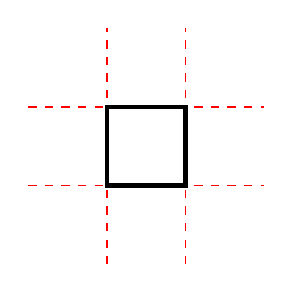
\begin{tikzpicture}[x=5mm, y=5mm]
 	\draw [red, dashed] (-3,1) -- (3,1);
	\draw [red, dashed] (-3,-1) -- (3,-1);
	\draw [red, dashed] (-1,-3) -- (-1,3);
	\draw [red, dashed] (1,-3) -- (1,3);
	\draw [ultra thick] (1,1) rectangle (-1,-1);
 \end{tikzpicture}
 &
 Each of these red dashed lines divides the plane into ``inner'' and ``outer'' sections.

\end{tabular}
 
\begin{tabular}{m{90mm}m{60mm}} 
 \begin{tikzpicture}[x=15mm, y=15mm]
 	\draw [red, dashed] (-3,1) -- (3,1);
	\draw [red, dashed] (-3,-1) -- (3,-1);
	\draw [red, dashed] (-1,-3) -- (-1,3);
	\draw [red, dashed] (1,-3) -- (1,3);
	\draw [ultra thick] (1,1) rectangle (-1,-1);
	\path (0,0) node {\tt 0000};
	\path (-2,2) node {\tt 1001};
	\path (0,2) node {\tt 1000};
	\path (2,2) node {\tt 1010};
	\path (-2,0) node {\tt 0001};
	\path (2,0) node {\tt 0010};
	\path (-2,-2) node {\tt 0101};
	\path (0,-2) node {\tt 0100};
	\path (2,-2) node {\tt 0110};
 \end{tikzpicture}
 &
 {\bf Encoding}

{\it Region out-codes}

\
 
 Pick an order (and be consistent)
 
 \
 
Dr. Borst's order in today's class:  Top, Bottom, Right, Left

\

Encode each sector with a four-digit binary code in which each digit tells whether the points are inside (0) or outside (1) the boundary.

\

``On the line'' counts as inside.  

 \end{tabular}
 
\begin{tabular}{m{60mm}m{90mm}} 

{\bf Iterative Algorithm}

Assign codes to segment endpoints.

\

{\tt IF} the segment is entirely in the window (both codes {\tt 0000})

\qquad Accept the segment

\

{\tt ELIF} both endpoints are outside a common boundary, {\it e.g.} both to the left, {\it i.e.} logical {\tt AND} of codes is nonzero,

\qquad Reject the segment.

\qquad (Same as culling.)

\

{\tt ELSE}  

\qquad Cut segment at a boundary

\qquad Discard the outer part

\qquad Run C-S Clipper on the inner part.  

&
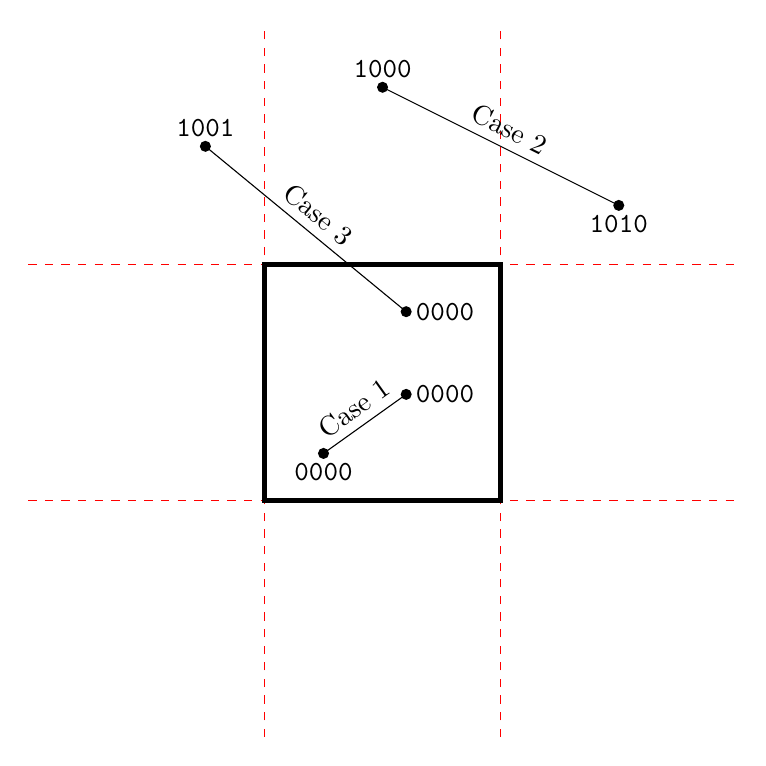
\begin{tikzpicture}[x=1.5mm, y=1.5mm]
 	\draw [red, dashed] (-30,10) -- (30,10);
	\draw [red, dashed] (-30,-10) -- (30,-10);
	\draw [red, dashed] (-10,-30) -- (-10,30);
	\draw [red, dashed] (10,-30) -- (10,30);
	\draw [ultra thick] (10,10) rectangle (-10,-10);

	\coordinate (A) at (-5,-6);
	\coordinate (B) at (2,-1);
	\fill (A) circle (2pt) node [below] {\tt 0000};
	\fill (B) circle (2pt) node [right] {\tt 0000};
	\draw (A) -- (B);
	\path (A) -- (B) node [midway, sloped, above] {Case 1};

	\coordinate (C) at (0,25);
	\coordinate (D) at (20,15);
	\fill (C) circle (2pt) node [above] {\tt 1000};
	\fill (D) circle (2pt) node [below] {\tt 1010};
	\draw (C) -- (D);
	\path (C) -- (D) node [midway, sloped, above] {Case 2};

	\coordinate (E) at (-15,20);
	\coordinate (F) at (2,6);
	\fill (E) circle (2pt) node [above] {\tt 1001};
	\fill (F) circle (2pt) node [right] {\tt 0000};
	\draw (E) -- (F) node [midway, sloped, above] {Case 3};

 \end{tikzpicture}
 \end{tabular}
 
{\bf To Cut the Line}

Pick an outside (not {\tt 0000}) endpoint.

Walk through the four digits left to right.

Identify the first nonzero bit in the code.

Cut the line at the boundary that corresponds to that bit.  

Lather, rinse, repeat.  

\

\begin{tabular}{@{}m{90mm}m{60mm}} 

1.  Scan the point codes left to right and pick the first one with a {\tt 1}.  There will be only one, because if they both had a {\tt 1} in the same position, they would have already been eliminated as being outside the same boundary.  Choose {\tt 1010}.

&
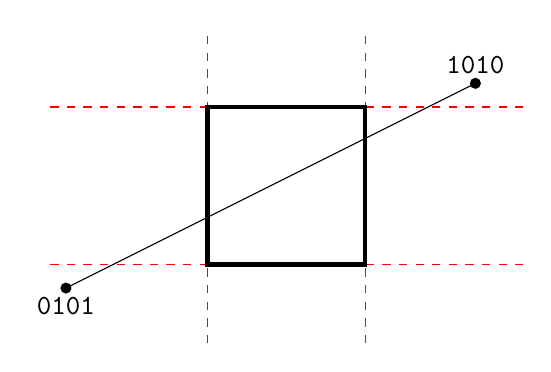
\begin{tikzpicture}[x=1.0mm, y=1.0mm]
 	\draw [red, dashed] (-30,10) -- (30,10);
	\draw [red, dashed] (-30,-10) -- (30,-10);
	\draw [red, dashed] (-10,-20) -- (-10,20);
	\draw [red, dashed] (10,-20) -- (10,20);
	\draw [ultra thick] (10,10) rectangle (-10,-10);

	\coordinate (A) at (-28,-13);
	\coordinate (B) at (24,13);
	\fill (A) circle (2pt) node [below] {\tt 0101};
	\fill (B) circle (2pt) node [above] {\tt 1010};
	\draw (A) -- (B);
	
	\coordinate (C) at (-22,-10);
	\coordinate (D) at (-10,-4);
	\coordinate (E) at (10,6);
	\coordinate (F) at (18,10);
	
%	\fill (C) circle (2pt) node [above left] {\tt 0001};
%	\fill (D) circle (2pt) node [above left] {\tt 0000};
%	\fill (E) circle (2pt) node [below right] {\tt 0000};
%	\fill (F) circle (2pt) node [below right] {\tt 0010};

 \end{tikzpicture}
 \end{tabular}
 
\

\begin{tabular}{@{}m{90mm}m{60mm}} 

2.  In {\tt 1010}, scan left to right to find the first {\tt 1}, which here represents ``Top."  Cut at the top boundary.  

\

3.  Check to see whether both points have encoding {\tt 0000}.  If they do, accept and end.   If not, check to see whether the encodings of the two points share a {\tt 1}.  If they do, reject the line.  

\

4.  Scan the point codes left to right and pick the first one with a {\tt 1}.  Choose {\tt 0101}.


&
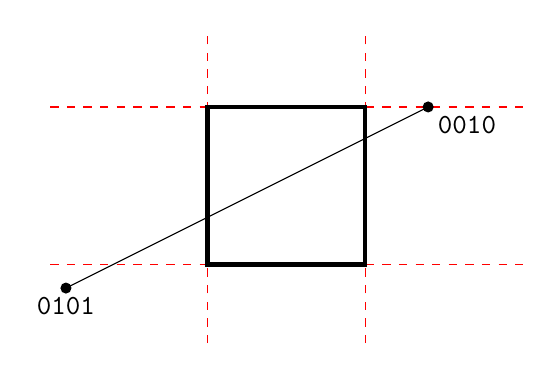
\begin{tikzpicture}[x=1.0mm, y=1.0mm]
 	\draw [red, dashed] (-30,10) -- (30,10);
	\draw [red, dashed] (-30,-10) -- (30,-10);
	\draw [red, dashed] (-10,-20) -- (-10,20);
	\draw [red, dashed] (10,-20) -- (10,20);
	\draw [ultra thick] (10,10) rectangle (-10,-10);

	\coordinate (A) at (-28,-13);
	\coordinate (B) at (24,13);
	\coordinate (C) at (-22,-10);
	\coordinate (D) at (-10,-4);
	\coordinate (E) at (10,6);
	\coordinate (F) at (18,10);
	
	\fill (A) circle (2pt) node [below] {\tt 0101};
%	\fill (C) circle (2pt) node [above left] {\tt 0001};
%	\fill (D) circle (2pt) node [above left] {\tt 0000};
%	\fill (E) circle (2pt) node [below right] {\tt 0000};
	\fill (F) circle (2pt) node [below right] {\tt 0010};
%	\fill (B) circle (2pt) node [above] {\tt 1010};

	\draw (A) -- (F);
	

 \end{tikzpicture}
 \end{tabular}
 
\

\begin{tabular}{@{}m{90mm}m{60mm}} 

5.  In {\tt 0101}, scan left to right to find the first {\tt 1}, which here represents ``Bottom."  Cut at the bottom boundary.  

\

6.  Check to see whether both points have encoding {\tt 0000}.  If they do, accept and end.  If not, check to see whether the encodings of the two points share a {\tt 1}.  If they do, reject the line.  

\

7.  Scan the point codes left to right and pick the first one with a {\tt 1}.  Choose {\tt 0010}.


&
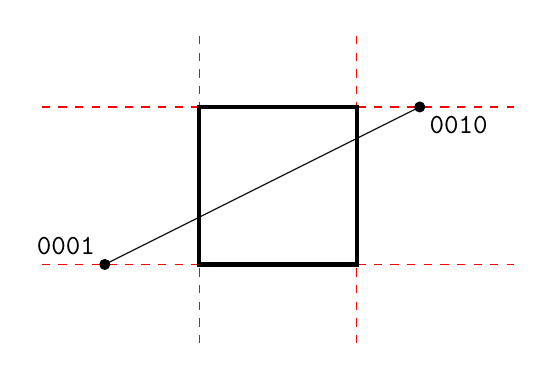
\begin{tikzpicture}[x=1.0mm, y=1.0mm]
 	\draw [red, dashed] (-30,10) -- (30,10);
	\draw [red, dashed] (-30,-10) -- (30,-10);
	\draw [red, dashed] (-10,-20) -- (-10,20);
	\draw [red, dashed] (10,-20) -- (10,20);
	\draw [ultra thick] (10,10) rectangle (-10,-10);

	\coordinate (A) at (-28,-13);
	\coordinate (B) at (24,13);
	\coordinate (C) at (-22,-10);
	\coordinate (D) at (-10,-4);
	\coordinate (E) at (10,6);
	\coordinate (F) at (18,10);
	
%	\fill (A) circle (2pt) node [below] {\tt 0101};
	\fill (C) circle (2pt) node [above left] {\tt 0001};
%	\fill (D) circle (2pt) node [above left] {\tt 0000};
%	\fill (E) circle (2pt) node [below right] {\tt 0000};
	\fill (F) circle (2pt) node [below right] {\tt 0010};
%	\fill (B) circle (2pt) node [above] {\tt 1010};

	\draw (C) -- (F);
	

 \end{tikzpicture}
 \end{tabular}
 
\

\begin{tabular}{@{}m{90mm}m{60mm}} 

8.  In {\tt 0010}, scan left to right to find the first {\tt 1}, which here represents ``Right."  Cut at the right boundary.  

\

9.  Check to see whether both points have encoding {\tt 0000}.  If they do, accept and end.  If not, check to see whether the encodings of the two points share a {\tt 1}.  If they do, reject the line.  

\

10.  Scan the point codes left to right and pick the first one with a {\tt 1}.  Choose {\tt 0001}.


&
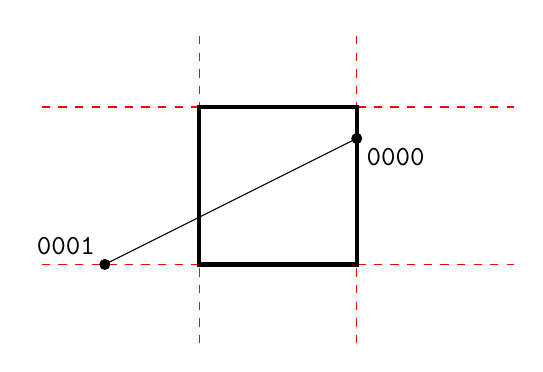
\begin{tikzpicture}[x=1.0mm, y=1.0mm]
 	\draw [red, dashed] (-30,10) -- (30,10);
	\draw [red, dashed] (-30,-10) -- (30,-10);
	\draw [red, dashed] (-10,-20) -- (-10,20);
	\draw [red, dashed] (10,-20) -- (10,20);
	\draw [ultra thick] (10,10) rectangle (-10,-10);

	\coordinate (A) at (-28,-13);
	\coordinate (B) at (24,13);
	\coordinate (C) at (-22,-10);
	\coordinate (D) at (-10,-4);
	\coordinate (E) at (10,6);
	\coordinate (F) at (18,10);
	
%	\fill (A) circle (2pt) node [below] {\tt 0101};
	\fill (C) circle (2pt) node [above left] {\tt 0001};
%	\fill (D) circle (2pt) node [above left] {\tt 0000};
	\fill (E) circle (2pt) node [below right] {\tt 0000};
%	\fill (F) circle (2pt) node [below right] {\tt 0010};
%	\fill (B) circle (2pt) node [above] {\tt 1010};

	\draw (C) -- (E);
	

 \end{tikzpicture}
 \end{tabular}
 
\

\

\begin{tabular}{@{}m{90mm}m{60mm}} 

11.  In {\tt 0001}, scan left to right to find the first {\tt 1}, which here represents ``Left."  Cut at the left boundary.  

\

12.  Check to see whether both points have encoding {\tt 0000}.  Since they do, accept and end.  

\



&
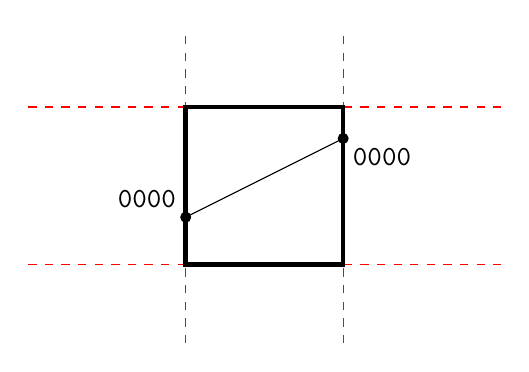
\begin{tikzpicture}[x=1.0mm, y=1.0mm]
 	\draw [red, dashed] (-30,10) -- (30,10);
	\draw [red, dashed] (-30,-10) -- (30,-10);
	\draw [red, dashed] (-10,-20) -- (-10,20);
	\draw [red, dashed] (10,-20) -- (10,20);
	\draw [ultra thick] (10,10) rectangle (-10,-10);

	\coordinate (A) at (-28,-13);
	\coordinate (B) at (24,13);
	\coordinate (C) at (-22,-10);
	\coordinate (D) at (-10,-4);
	\coordinate (E) at (10,6);
	\coordinate (F) at (18,10);
	
%	\fill (A) circle (2pt) node [below] {\tt 0101};
%	\fill (C) circle (2pt) node [above left] {\tt 0001};
	\fill (D) circle (2pt) node [above left] {\tt 0000};
	\fill (E) circle (2pt) node [below right] {\tt 0000};
%	\fill (F) circle (2pt) node [below right] {\tt 0010};
%	\fill (B) circle (2pt) node [above] {\tt 1010};

	\draw (D) -- (E);
	

 \end{tikzpicture}
 \end{tabular}
 
\

Generalizes to 3D.  

\subsection{Clipping Polygons}

{\color{red} Not clear about what to do with each vertex in the algorithm, whether to discard it or not.}

\

{\color{red} Dr. Borst's comment:  I think of it as building a new description of a polygon, not modifying (e.g., discarding) in the original description. Then the choices are copying a vertex to the new description, ignoring the vertex and moving on, adding a new computed intersection coord to the output list, or adding an intersection coord plus a copied vertex.}

\

The math is a little more tedious, but not much.  

Window must be convex.

Formal mathematical definition of {\it convex polygon}:  A polygon is convex iff, given any two points in the interior, all of the points on the segment connecting the points are in the interior.  

Convex casual definition:  If a bug walking around the perimeter only turns one way, it's convex.  

\

\begin{tabular}{m{75mm}m{85mm}}
\begin{tikzpicture}[x=1.5mm,y=1.5mm]

	\coordinate (TL) at (-30,10);
	\coordinate (TR) at (20,10);
	\coordinate (BL) at (-30,-10);
	\coordinate (BR) at (20,-10);
	\coordinate (LB) at (-10,-20);
	\coordinate (LT) at (-10,30);
	\coordinate (RB) at (10,-20);
	\coordinate (RT) at (10,30);

 	\draw [red, dashed] (TL) -- (TR);
	\draw [red, dashed] (BL) -- (BR);
	\draw [red, dashed] (LB) -- (LT);
	\draw [red, dashed] (RB) -- (RT);
	\draw [ultra thick] (10,10) rectangle (-10,-10);
	
	\coordinate (v0) at ({-5+20*cos(90+0*36)},{8+20*sin(90+0*36)});
	\coordinate (v1) at ({-5+ 7*cos(90+1*36)},{8+ 7*sin(90+1*36)});
	\coordinate (v2) at ({-5+20*cos(90+2*36)},{8+20*sin(90+2*36)});
	\coordinate (v3) at ({-5+ 7*cos(90+3*36)},{8+ 7*sin(90+3*36)});
	\coordinate (v4) at ({-5+20*cos(90+4*36)},{8+20*sin(90+4*36)});
	\coordinate (v5) at ({-5+ 7*cos(90+5*36)},{8+ 7*sin(90+5*36)});
	\coordinate (v6) at ({-5+20*cos(90+6*36)},{8+20*sin(90+6*36)});
	\coordinate (v7) at ({-5+ 7*cos(90+7*36)},{8+ 7*sin(90+7*36)});
	\coordinate (v8) at ({-5+20*cos(90+8*36)},{8+20*sin(90+8*36)});
	\coordinate (v9) at ({-5+ 7*cos(90+9*36)},{8+ 7*sin(90+9*36)});
	
	\path ($1.1*(v0)-0.1*(-5,8)$) node {\tt v0};
	\path ($1.4*(v1)-0.4*(-5,8)$) node {\tt v1};
	\path ($1.1*(v2)-0.1*(-5,8)$) node {\tt v2};
	\path ($1.4*(v3)-0.4*(-5,8)$) node {\tt v3};
	\path ($1.1*(v4)-0.1*(-5,8)$) node {\tt v4};
	\path ($1.4*(v5)-0.4*(-5,8)$) node {\tt v5};
	\path ($1.1*(v6)-0.1*(-5,8)$) node {\tt v6};
	\path ($1.4*(v7)-0.4*(-5,8)$) node {\tt v7};
	\path ($1.1*(v8)-0.1*(-5,8)$) node {\tt v8};
	\path ($1.4*(v9)-0.4*(-5,8)$) node {\tt v9};
	
	\draw [blue, ultra thick] (v0) -- (v1) -- (v2) -- (v3) -- (v4) -- (v5) -- (v6) -- (v7) -- (v8) -- (v9) -- (v0);

\end{tikzpicture}
&
{\bf Algorithm}

Pick a boundary line.

Walk around in one direction, slicing the segments that intersect the boundary line.  

\

Top

{\tt v0 -- v1} is outside. Discard {\tt v0}.

{\tt v1 -- v2} is outside. Discard {\tt v1}.  

{\tt v2 -- v3} goes outside to inside. Make {\tt v10} at intersection.  Discard {\tt v2}.  

{\tt v3 -- v4} is inside.   Keep these vertices.  

$\vdots$

{\tt v7 -- v8} intersects.  Make {\tt v11} at intersection.  

\end{tabular}

New polygon is {\tt v10 -- v3 -- v4 -- v5 -- v6 -- v7 -- v11}

\begin{tabular}{m{100mm}m{60mm}}
\begin{tikzpicture}[x=1.5mm,y=1.5mm]

	\coordinate (TL) at (-30,10);
	\coordinate (TR) at (20,10);
	\coordinate (BL) at (-30,-10);
	\coordinate (BR) at (20,-10);
	\coordinate (LB) at (-10,-20);
	\coordinate (LT) at (-10,30);
	\coordinate (RB) at (10,-20);
	\coordinate (RT) at (10,30);

 	\draw [red, dashed] (TL) -- (TR);
	\draw [red, dashed] (BL) -- (BR);
	\draw [red, dashed] (LB) -- (LT);
	\draw [red, dashed] (RB) -- (RT);
	\draw [ultra thick] (10,10) rectangle (-10,-10);
	
	\coordinate (v0) at ({-5+20*cos(90+0*36)},{8+20*sin(90+0*36)});
	\coordinate (v1) at ({-5+ 7*cos(90+1*36)},{8+ 7*sin(90+1*36)});
	\coordinate (v2) at ({-5+20*cos(90+2*36)},{8+20*sin(90+2*36)});
	\coordinate (v3) at ({-5+ 7*cos(90+3*36)},{8+ 7*sin(90+3*36)});
	\coordinate (v4) at ({-5+20*cos(90+4*36)},{8+20*sin(90+4*36)});
	\coordinate (v5) at ({-5+ 7*cos(90+5*36)},{8+ 7*sin(90+5*36)});
	\coordinate (v6) at ({-5+20*cos(90+6*36)},{8+20*sin(90+6*36)});
	\coordinate (v7) at ({-5+ 7*cos(90+7*36)},{8+ 7*sin(90+7*36)});
	\coordinate (v8) at ({-5+20*cos(90+8*36)},{8+20*sin(90+8*36)});
	\coordinate (v9) at ({-5+ 7*cos(90+9*36)},{8+ 7*sin(90+9*36)});
	
	\coordinate (v10) at (intersection of TL--TR and v2--v3);
	\coordinate (v11) at (intersection of TL--TR and v7--v8);

	
	\path ($1.1*(v0)-0.1*(-5,8)$) node {\tt v0};
	\path ($1.4*(v1)-0.4*(-5,8)$) node {\tt v1};
	\path ($1.1*(v2)-0.1*(-5,8)$) node {\tt v2};
	\path ($1.4*(v3)-0.4*(-5,8)$) node {\tt v3};
	\path ($1.1*(v4)-0.1*(-5,8)$) node {\tt v4};
	\path ($1.4*(v5)-0.4*(-5,8)$) node {\tt v5};
	\path ($1.1*(v6)-0.1*(-5,8)$) node {\tt v6};
	\path ($1.4*(v7)-0.4*(-5,8)$) node {\tt v7};
	\path ($1.1*(v8)-0.1*(-5,8)$) node {\tt v8};
	\path ($1.4*(v9)-0.4*(-5,8)$) node {\tt v9};
	
	\path ($(v10)+(1,2)$) node {\tt v10};
	\path ($(v11)+(-1,2)$) node {\tt v11};
	
	\draw [blue, dashed] (v0) -- (v1) -- (v2) -- (v3) -- (v4) -- (v5) -- (v6) -- (v7) -- (v8) -- (v9) -- (v0);
	\draw [blue, ultra thick] (v10) -- (v3) -- (v4) -- (v5) -- (v6) -- (v7) -- (v11) -- (v10);

\end{tikzpicture}
&

Repeat for other three boundary lines.  
\end{tabular}

\

Four cases moving from one vertex to the next.  

\begin{enumerate}
	\item Completely inside.  Add one vertex
	\item Crosses inside to outside.  Add one vertex.  
	\item Completely outside.  Do nothing.
	\item Cross outside to inside.  Add two vertices.  
\end{enumerate}

